\documentclass{standalone}
\usepackage{tikz}
\usetikzlibrary{patterns, positioning}


\begin{document}
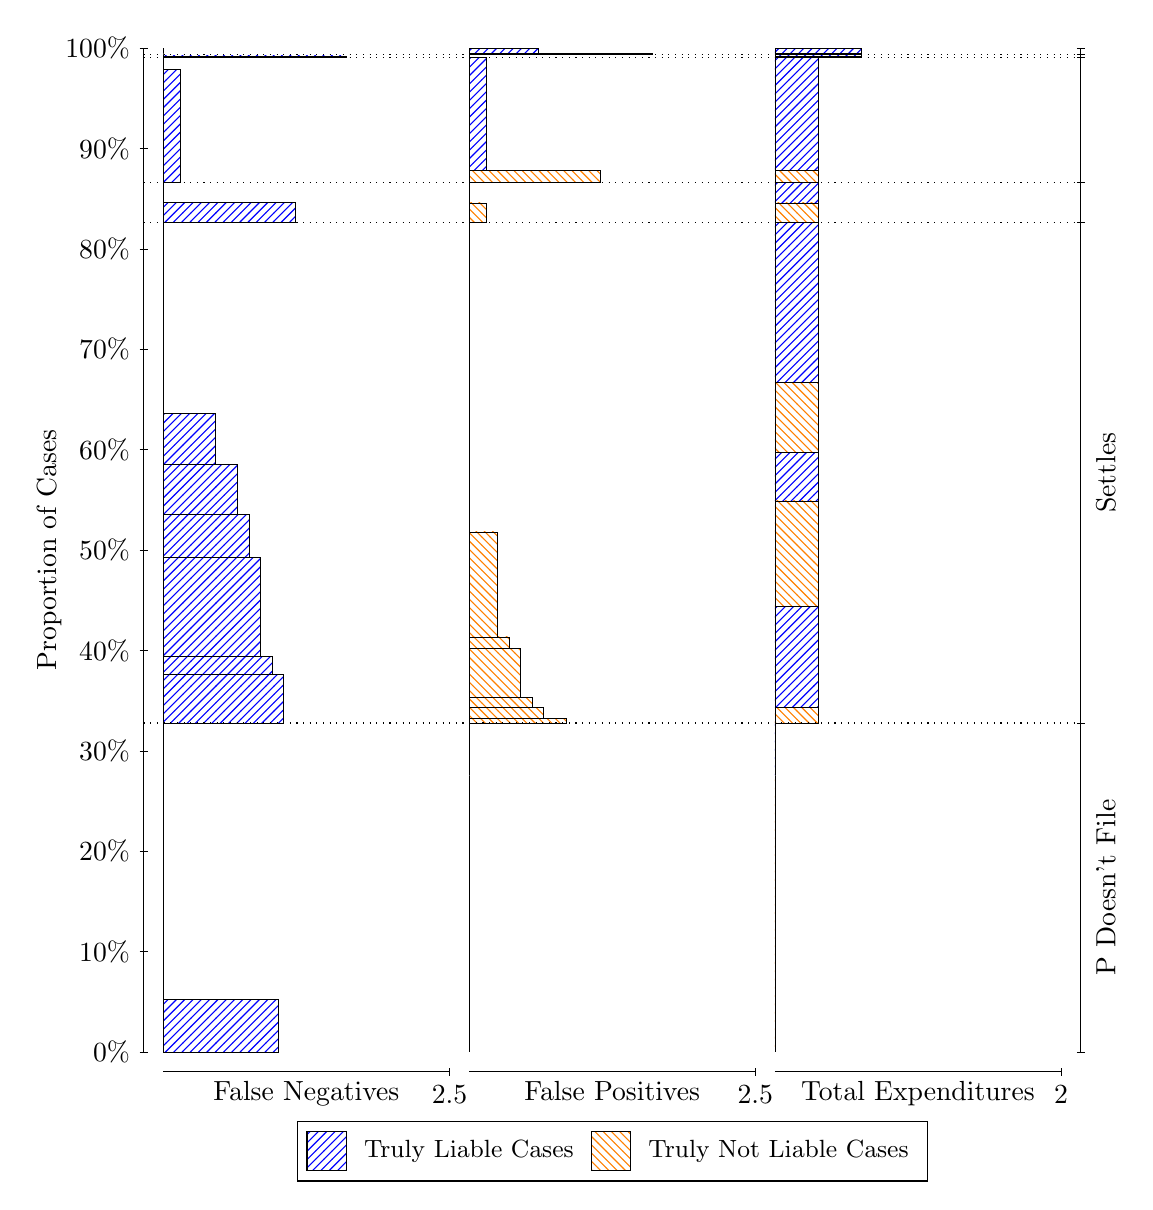
\begin{tikzpicture}
\draw[black, very thin] (1.5,1.75) -- (1.5,14.5);
\node[rotate=90, text=black, anchor=center] at (0.3, 8.125) {Proportion of Cases};
\draw[black, very thin] (1.45,1.75) -- (1.55,1.75);
\node[text=black, anchor=east] at (1.45, 1.75) {0\%};
\draw[black, very thin] (1.45,3.025) -- (1.55,3.025);
\node[text=black, anchor=east] at (1.45, 3.025) {10\%};
\draw[black, very thin] (1.45,4.3) -- (1.55,4.3);
\node[text=black, anchor=east] at (1.45, 4.3) {20\%};
\draw[black, very thin] (1.45,5.575) -- (1.55,5.575);
\node[text=black, anchor=east] at (1.45, 5.575) {30\%};
\draw[black, very thin] (1.45,6.85) -- (1.55,6.85);
\node[text=black, anchor=east] at (1.45, 6.85) {40\%};
\draw[black, very thin] (1.45,8.125) -- (1.55,8.125);
\node[text=black, anchor=east] at (1.45, 8.125) {50\%};
\draw[black, very thin] (1.45,9.4) -- (1.55,9.4);
\node[text=black, anchor=east] at (1.45, 9.4) {60\%};
\draw[black, very thin] (1.45,10.675) -- (1.55,10.675);
\node[text=black, anchor=east] at (1.45, 10.675) {70\%};
\draw[black, very thin] (1.45,11.95) -- (1.55,11.95);
\node[text=black, anchor=east] at (1.45, 11.95) {80\%};
\draw[black, very thin] (1.45,13.225) -- (1.55,13.225);
\node[text=black, anchor=east] at (1.45, 13.225) {90\%};
\draw[black, very thin] (1.45,14.5) -- (1.55,14.5);
\node[text=black, anchor=east] at (1.45, 14.5) {100\%};

\draw[black, very thin] (13.4,1.75) -- (13.4,14.5);
\draw[black, very thin] (13.35,1.75) -- (13.45,1.75);
\node[anchor=west] at (13.35, 1.75) {};
\draw[black, very thin] (13.35,5.9277) -- (13.45,5.9277);
\node[anchor=west] at (13.35, 5.9277) {};
\draw[black, very thin] (13.35,12.287) -- (13.45,12.287);
\node[anchor=west] at (13.35, 12.287) {};
\draw[black, very thin] (13.35,12.79) -- (13.45,12.79);
\node[anchor=west] at (13.35, 12.79) {};
\draw[black, very thin] (13.35,14.381) -- (13.45,14.381);
\node[anchor=west] at (13.35, 14.381) {};
\draw[black, very thin] (13.35,14.415) -- (13.45,14.415);
\node[anchor=west] at (13.35, 14.415) {};
\draw[black, very thin] (13.35,14.5) -- (13.45,14.5);
\node[anchor=west] at (13.35, 14.5) {};

\draw[black, very thin, pattern color=blue, pattern=north east lines] (1.75,1.75) rectangle (3.2033,2.4162);
\draw[black, very thin, pattern color=orange, pattern=north west lines] (1.75,2.4162) rectangle (1.75,5.9277);
\draw[black, very thin, pattern color=blue, pattern=north east lines] (1.75,5.9277) rectangle (3.276,6.5414);
\draw[black, very thin, pattern color=blue, pattern=north east lines] (1.75,6.5414) rectangle (3.1307,6.7772);
\draw[black, very thin, pattern color=blue, pattern=north east lines] (1.75,6.7772) rectangle (2.9853,8.0344);
\draw[black, very thin, pattern color=blue, pattern=north east lines] (1.75,8.0344) rectangle (2.84,8.5755);
\draw[black, very thin, pattern color=blue, pattern=north east lines] (1.75,8.5755) rectangle (2.6947,9.2144);
\draw[black, very thin, pattern color=blue, pattern=north east lines] (1.75,9.2144) rectangle (2.404,9.8586);
\draw[black, very thin, pattern color=orange, pattern=north west lines] (1.75,9.8586) rectangle (1.75,12.287);
\draw[black, very thin, pattern color=blue, pattern=north east lines] (1.75,12.287) rectangle (3.4213,12.544);
\draw[black, very thin, pattern color=orange, pattern=north west lines] (1.75,12.544) rectangle (1.75,12.79);
\draw[black, very thin, pattern color=blue, pattern=north east lines] (1.75,12.79) rectangle (1.968,14.227);
\draw[black, very thin, pattern color=orange, pattern=north west lines] (1.75,14.227) rectangle (1.75,14.381);
\draw[black, very thin, pattern color=blue, pattern=north east lines] (1.75,14.381) rectangle (4.0753,14.399);
\draw[black, very thin, pattern color=orange, pattern=north west lines] (1.75,14.399) rectangle (1.75,14.415);
\draw[black, very thin, pattern color=orange, pattern=north west lines] (1.75,14.415) rectangle (1.75,14.433);
\draw[black, very thin, pattern color=blue, pattern=north east lines] (1.75,14.433) rectangle (1.75,14.5);
\draw[black, very thin, pattern color=orange, pattern=north west lines] (5.6333,1.75) rectangle (5.6333,5.2615);
\draw[black, very thin, pattern color=blue, pattern=north east lines] (5.6333,5.2615) rectangle (5.6333,5.9277);
\draw[black, very thin, pattern color=orange, pattern=north west lines] (5.6333,5.9277) rectangle (6.8687,5.9891);
\draw[black, very thin, pattern color=orange, pattern=north west lines] (5.6333,5.9891) rectangle (6.578,6.1302);
\draw[black, very thin, pattern color=orange, pattern=north west lines] (5.6333,6.1302) rectangle (6.4327,6.2503);
\draw[black, very thin, pattern color=orange, pattern=north west lines] (5.6333,6.2503) rectangle (6.2873,6.8729);
\draw[black, very thin, pattern color=orange, pattern=north west lines] (5.6333,6.8729) rectangle (6.142,7.0222);
\draw[black, very thin, pattern color=orange, pattern=north west lines] (5.6333,7.0222) rectangle (5.9967,8.3563);
\draw[black, very thin, pattern color=blue, pattern=north east lines] (5.6333,8.3563) rectangle (5.6333,12.287);
\draw[black, very thin, pattern color=orange, pattern=north west lines] (5.6333,12.287) rectangle (5.8513,12.533);
\draw[black, very thin, pattern color=blue, pattern=north east lines] (5.6333,12.533) rectangle (5.6333,12.79);
\draw[black, very thin, pattern color=orange, pattern=north west lines] (5.6333,12.79) rectangle (7.3047,12.944);
\draw[black, very thin, pattern color=blue, pattern=north east lines] (5.6333,12.944) rectangle (5.8513,14.381);
\draw[black, very thin, pattern color=orange, pattern=north west lines] (5.6333,14.381) rectangle (5.6333,14.397);
\draw[black, very thin, pattern color=blue, pattern=north east lines] (5.6333,14.397) rectangle (5.6333,14.415);
\draw[black, very thin, pattern color=orange, pattern=north west lines] (5.6333,14.415) rectangle (7.9587,14.433);
\draw[black, very thin, pattern color=blue, pattern=north east lines] (5.6333,14.433) rectangle (6.5053,14.5);
\draw[black, very thin, pattern color=orange, pattern=north west lines] (9.5167,1.75) rectangle (9.5167,5.2615);
\draw[black, very thin, pattern color=blue, pattern=north east lines] (9.5167,5.2615) rectangle (9.5167,5.9277);
\draw[black, very thin, pattern color=orange, pattern=north west lines] (9.5167,5.9277) rectangle (10.062,6.1302);
\draw[black, very thin, pattern color=blue, pattern=north east lines] (9.5167,6.1302) rectangle (10.062,7.4134);
\draw[black, very thin, pattern color=orange, pattern=north west lines] (9.5167,7.4134) rectangle (10.062,8.7475);
\draw[black, very thin, pattern color=blue, pattern=north east lines] (9.5167,8.7475) rectangle (10.062,9.3612);
\draw[black, very thin, pattern color=orange, pattern=north west lines] (9.5167,9.3612) rectangle (10.062,10.253);
\draw[black, very thin, pattern color=blue, pattern=north east lines] (9.5167,10.253) rectangle (10.062,12.287);
\draw[black, very thin, pattern color=orange, pattern=north west lines] (9.5167,12.287) rectangle (10.062,12.533);
\draw[black, very thin, pattern color=blue, pattern=north east lines] (9.5167,12.533) rectangle (10.062,12.79);
\draw[black, very thin, pattern color=orange, pattern=north west lines] (9.5167,12.79) rectangle (10.062,12.944);
\draw[black, very thin, pattern color=blue, pattern=north east lines] (9.5167,12.944) rectangle (10.062,14.381);
\draw[black, very thin, pattern color=orange, pattern=north west lines] (9.5167,14.381) rectangle (10.607,14.397);
\draw[black, very thin, pattern color=blue, pattern=north east lines] (9.5167,14.397) rectangle (10.607,14.415);
\draw[black, very thin, pattern color=orange, pattern=north west lines] (9.5167,14.415) rectangle (10.607,14.433);
\draw[black, very thin, pattern color=blue, pattern=north east lines] (9.5167,14.433) rectangle (10.607,14.5);
\draw[black, dotted] (1.5,5.9277) -- (13.4,5.9277);
\draw[black, dotted] (1.5,12.287) -- (13.4,12.287);
\draw[black, dotted] (1.5,12.79) -- (13.4,12.79);
\draw[black, dotted] (1.5,14.381) -- (13.4,14.381);
\draw[black, dotted] (1.5,14.415) -- (13.4,14.415);
\draw[black, very thin] (1.75,1.5) -- (5.3833,1.5);
\node[text=black, anchor=north] at (3.5667, 1.5) {False Negatives};
\draw[black, very thin] (5.3833,1.45) -- (5.3833,1.55);
\node[text=black, anchor=north] at (5.3833, 1.45) {2.5};

\draw[black, very thin] (5.6333,1.5) -- (9.2667,1.5);
\node[text=black, anchor=north] at (7.45, 1.5) {False Positives};
\draw[black, very thin] (9.2667,1.45) -- (9.2667,1.55);
\node[text=black, anchor=north] at (9.2667, 1.45) {2.5};

\draw[black, very thin] (9.5167,1.5) -- (13.15,1.5);
\node[text=black, anchor=north] at (11.333, 1.5) {Total Expenditures};
\draw[black, very thin] (13.15,1.45) -- (13.15,1.55);
\node[text=black, anchor=north] at (13.15, 1.45) {2};

\node[text=black, centered, rotate=90] at (13.72, 3.8389) {P Doesn't File};
\node[text=black, centered, rotate=90] at (13.72, 9.1075) {Settles};





\draw (7.449999999999999,1.5) node[draw=none] (baseCoordinate) {};
\begin{scope}[align=center]
        \matrix[scale=0.5, draw=black, below=0.5cm of baseCoordinate, nodes={draw}, column sep=0.1cm]{
            \node[rectangle, draw, minimum width=0.5cm, minimum height=0.5cm, pattern color=blue, pattern=north east lines] {}; &
            \node[draw=none, font=\small, text=black] (B) {Truly Liable Cases}; &
            \node[rectangle, draw, minimum width=0.5cm, minimum height=0.5cm, pattern color=orange, pattern=north west lines] {}; &
            \node[draw=none, font=\small, text=black] (B) {Truly Not Liable Cases}; \\
            };
\end{scope}

\end{tikzpicture}
\end{document}